% Created 2024-12-05 jue 20:18
% Intended LaTeX compiler: pdflatex
\documentclass[10pt]{article}
\usepackage[utf8]{inputenc}
\usepackage{lmodern}
\usepackage[T1]{fontenc}
\usepackage[top=1in, bottom=1.in, left=1in, right=1in]{geometry}
\usepackage{graphicx}
\usepackage{longtable}
\usepackage{float}
\usepackage{wrapfig}
\usepackage{rotating}
\usepackage[normalem]{ulem}
\usepackage{amsmath}
\usepackage{textcomp}
\usepackage{marvosym}
\usepackage{wasysym}
\usepackage{amssymb}
\usepackage{amsmath}
\usepackage[theorems, skins]{tcolorbox}
\usepackage[version=3]{mhchem}
\usepackage[numbers,super,sort&compress]{natbib}
\usepackage{natmove}
\usepackage{url}
\usepackage[cache=false]{minted}
\usepackage[strings]{underscore}
\usepackage[linktocpage,pdfstartview=FitH,colorlinks,
linkcolor=blue,anchorcolor=blue,
citecolor=blue,filecolor=blue,menucolor=blue,urlcolor=blue]{hyperref}
\usepackage{attachfile}
\usepackage{setspace}
\usepackage[spanish, ]{babel}
\usepackage{fontspec}
\date{}
\title{Tipos de interés a 3 y 6 meses en EEUU}
\begin{document}

\maketitle
\section*{Datos}
\label{sec:orgbd56a5c}

Datos semanales desde el 12 de diciembre de 1958 al 6 de agosto de
2004 (en total 2383 observaciones). \emph{Fuente}: ejemplo 8.6.5 del libro
de Ruey S. Tsay, \emph{Multivariate Time Series Analysis and its
applications} (\href{https://www.chicagobooth.edu/-/media/faculty/ruey-s-tsay/teaching/fts2/w-tb3n6ms.txt}{w-tb3n6ms.txt}).
\begin{description}
\item[{\texttt{TB3}}] 3-month Treasury Bill
\item[{\texttt{TB6}}] 6-month Treasury Bill
\end{description}


\begin{minted}[frame=lines,fontsize=\scriptsize,linenos=]{r}
open LetrasTesoroAmericano3y6meses.gdt
gnuplot TB3 TB6  --time-series --with-lines --output="TB3yTB6.png"
\end{minted}

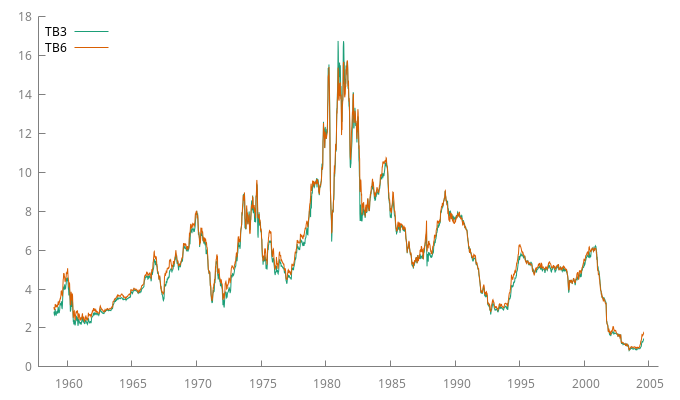
\includegraphics[width=0.35\textwidth]{./LetrasTesoroAmericano3y6meses/TB3yTB6.png}

\begin{itemize}
\item Ficheros \url{https://github.com/mbujosab/EconometriaAplicada-SRC/tree/main/Ejercicios}
\begin{itemize}
\item Versión en \href{https://github.com/mbujosab/EconometriaAplicada-SRC/blob/main/LetrasTesoroAmericano3y6meses.pdf}{pdf}
\item Datos: \url{LetrasTesoroAmericano3y6meses.gdt}
\item Guión de gretl: \url{LetrasTesoroAmericano3y6meses.inp}
\end{itemize}
\end{itemize}
\section*{Letras a tres meses}
\label{sec:orgaef2172}
\subsection*{Gráfico y correlograma de la serie temporal TB3}
\label{sec:org8d2996f}

\begin{minted}[frame=lines,fontsize=\scriptsize,linenos=]{r}
gnuplot TB3 --time-series --with-lines --output="TB3.png"
corrgm TB3 --plot="TB3ACF-PACF.png"
\end{minted}


\begin{center}
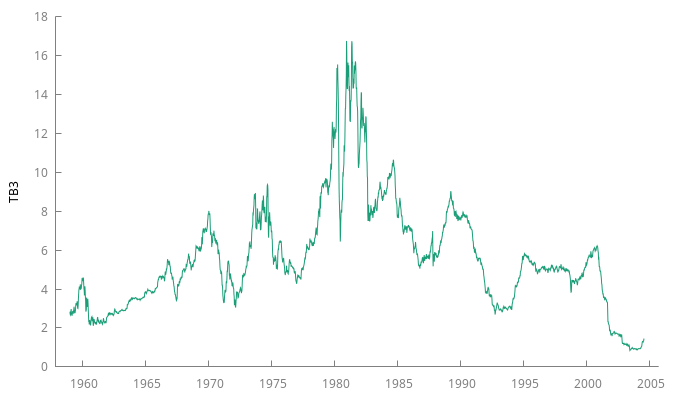
\includegraphics[width=0.5\textwidth]{./LetrasTesoroAmericano3y6meses/TB3.png}
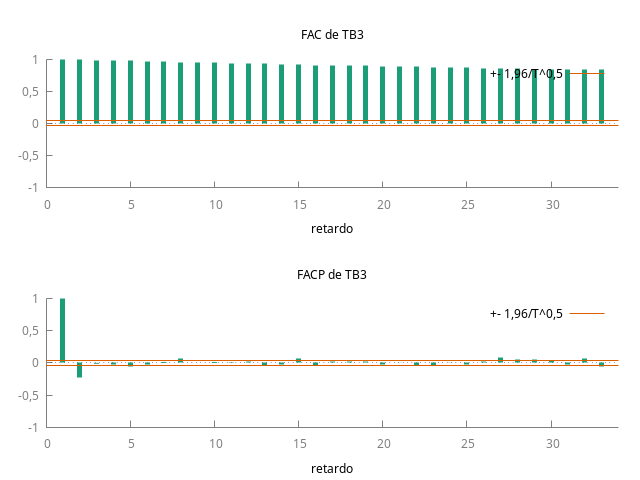
\includegraphics[width=0.4\textwidth]{./LetrasTesoroAmericano3y6meses/TB3ACF-PACF.png} 
\end{center}
\subsection*{Regresión auxiliar para TB3}
\label{sec:orga882c1a}

Consideremos la regresión $$\nabla TB3_{t} = \nu + \delta TB3_{t-1} +
\sum_{j=1}^3 \pi_j \nabla TB3_{t-j} + U_t.$$ Y consideremos la
siguiente hipótesis nula acerca del parámetro \(\delta\):
\begin{quote}
\(\,H_0: \delta = 0\), frente a \(H_1: \delta < 0\)
\end{quote}

\begin{minted}[frame=lines,fontsize=\scriptsize,linenos=]{r}
diff TB3
RegresionAUX_TB3 <- ols d_TB3 0 TB3(-1) d_TB3(-1) d_TB3(-2) d_TB3(-3) 
\end{minted}

{\footnotesize
\begin{verbatim}
Modelo 2: MCO, usando las observaciones 1959-01-09:2004-08-06 (T = 2379)
Variable dependiente: d_TB3

             coeficiente   Desv. típica   Estadístico t   valor p 
  ----------------------------------------------------------------
  const       0,0204353     0,00950288        2,150       0,0316   **
  TB3_1      -0,00371135    0,00152221       -2,438       0,0148   **
  d_TB3_1     0,271457      0,0204924        13,25        1,07e-38 ***
  d_TB3_2    -0,0148460     0,0212326        -0,6992      0,4845  
  d_TB3_3     0,0381931     0,0205139         1,862       0,0628   *

Media de la vble. dep. -0,000513   D.T. de la vble. dep.   0,212547
Suma de cuad. residuos  99,33579   D.T. de la regresión    0,204556
R-cuadrado              0,075335   R-cuadrado corregido    0,073777
F(4, 2374)              48,35422   Valor p (de F)          3,80e-39
Log-verosimilitud       402,1135   Criterio de Akaike     -794,2269
Criterio de Schwarz    -765,3547   Crit. de Hannan-Quinn  -783,7185
rho                    -0,002760   h de Durbin            -4,320544

Sin considerar la constante, el valor p más alto fue el de la variable 6 (d_TB3_2)
\end{verbatim}
}
\subsubsection*{Contraste de la hipótesis nula}
\label{sec:org9b646c5}

Respecto al contraste de la hipótesis nula sobre el parámetro \(\delta\)
de la anterior regresión auxiliar:
\begin{quote}
\(\,H_0: \delta = 0\), frente a \(H_1: \delta < 0\)
\end{quote}
Para el tamaño muestral considerado, y bajo la hipótesis nula, el
valor crítico del contraste para un nivel de significación del 5\% es
\texttt{-2.86}
\subsection*{Contraste aumentado de Dickey Fuller sobre la existencia de una raíz unitaria para TB3}
\label{sec:org058c624}

\begin{minted}[frame=lines,fontsize=\scriptsize,linenos=]{r}
adf 3 TB3 --c
\end{minted}

{\footnotesize
\begin{verbatim}
Contraste aumentado de Dickey-Fuller para TB3
incluyendo 3 retardos de (1-L)TB3
tamaño muestral 2379
la hipótesis nula de raíz unitaria es: [a = 1]

  contraste con constante 
  modelo: (1-L)y = b0 + (a-1)*y(-1) + ... + e
  valor estimado de (a - 1): -0,00371135
  estadístico de contraste: tau_c(1) = -2,43813
  valor p asintótico 0,1312
  Coef. de autocorrelación de primer orden de e: -0,003
  diferencias retardadas: F(3, 2374) = 63,404 [0,0000]
\end{verbatim}
}
\subsection*{Conteste KPSS de estacionariedad para TB3}
\label{sec:orgf022dca}

\begin{minted}[frame=lines,fontsize=\scriptsize,linenos=]{r}
kpss 3 TB3
\end{minted}

{\footnotesize
\begin{verbatim}
Contraste KPSS para TB3

T = 2383
Parámetro de truncamiento de los retardos = 3
Estadístico de contraste = 8,99282

                      10%      5%      1%
Valores críticos: 0,348   0,462   0,744
Valor p < .01
\end{verbatim}
}
\section*{Letras a seis meses}
\label{sec:org007c29c}
\subsection*{Gráfico y correlograma de la serie temporal TB6}
\label{sec:org170f783}

\begin{minted}[frame=lines,fontsize=\scriptsize,linenos=]{r}
gnuplot TB6 --time-series --with-lines --output="TB6.png"
corrgm TB6 --plot="TB6ACF-PACF.png"
\end{minted}


\begin{center}
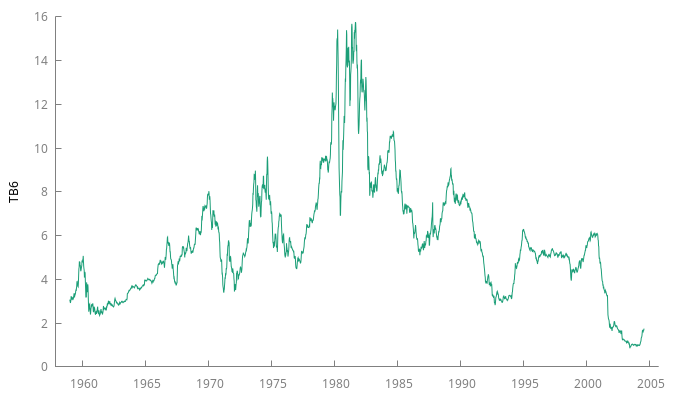
\includegraphics[width=0.5\textwidth]{./LetrasTesoroAmericano3y6meses/TB6.png} 
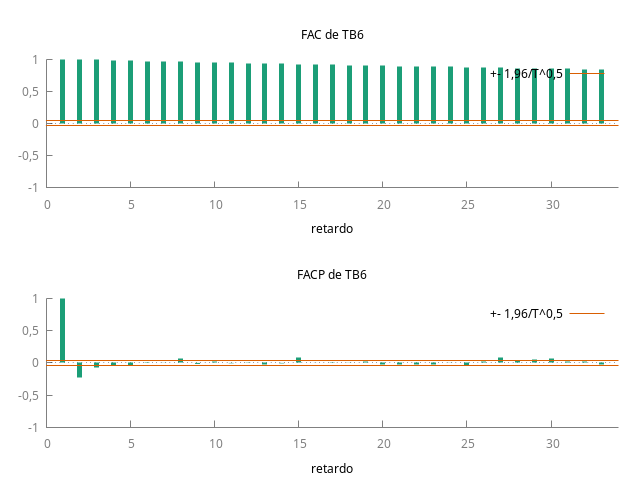
\includegraphics[width=0.4\textwidth]{./LetrasTesoroAmericano3y6meses/TB6ACF-PACF.png} 
\end{center}
\subsection*{Regresión auxiliar para TB6}
\label{sec:orgc3fb817}

Consideremos la regresión $$\nabla TB6_{t} = \nu + \delta TB6_{t-1} +
\sum_{j=1}^3 \pi_j \nabla TB6_{t-j} + U_t.$$ Y consideremos la
siguiente hipótesis nula acerca del parámetro \(\delta\):
\begin{quote}
\(\,H_0: \delta = 0\), frente a \(H_1: \delta < 0\)
\end{quote}

\begin{minted}[frame=lines,fontsize=\scriptsize,linenos=]{r}
diff TB6
RegresionAUX_TB6 <- ols d_TB6 0 TB6(-1) d_TB6(-1) d_TB6(-2) d_TB6(-3) 
\end{minted}

{\footnotesize
\begin{verbatim}
Modelo 4: MCO, usando las observaciones 1959-01-09:2004-08-06 (T = 2379)
Variable dependiente: d_TB6

             coeficiente   Desv. típica   Estadístico t   valor p 
  ----------------------------------------------------------------
  const       0,0188423     0,00868102        2,171       0,0301   **
  TB6_1      -0,00332840    0,00136431       -2,440       0,0148   **
  d_TB6_1     0,273770      0,0204870        13,36        2,52e-39 ***
  d_TB6_2     0,0535491     0,0212198         2,524       0,0117   **
  d_TB6_3     0,0408834     0,0205125         1,993       0,0464   **

Media de la vble. dep. -0,000509   D.T. de la vble. dep.   0,189439
Suma de cuad. residuos  77,37722   D.T. de la regresión    0,180537
R-cuadrado              0,093303   R-cuadrado corregido    0,091775
F(4, 2374)              61,07380   Valor p (de F)          3,60e-49
Log-verosimilitud       699,2666   Criterio de Akaike     -1388,533
Criterio de Schwarz    -1359,661   Crit. de Hannan-Quinn  -1378,025
rho                    -0,001784   h de Durbin            -2,253222
\end{verbatim}
}
\subsubsection*{Contraste de la hipótesis nula}
\label{sec:org64d1170}

Respecto al contraste de la hipótesis nula sobre el parámetro \(\delta\)
de la anterior regresión auxiliar:
\begin{quote}
\(\,H_0: \delta = 0\), frente a \(H_1: \delta < 0\)
\end{quote}
Para el tamaño muestral considerado, y bajo la hipótesis nula, el
valor crítico del contraste para un nivel de significación del 5\% es
\texttt{-2.86}
\subsection*{Contraste aumentado de Dickey Fuller sobre la existencia de una raíz unitaria para TB6}
\label{sec:org5b9af83}

\begin{minted}[frame=lines,fontsize=\scriptsize,linenos=]{r}
adf 3 TB6 --c
\end{minted}

{\footnotesize
\begin{verbatim}
Contraste aumentado de Dickey-Fuller para TB6
incluyendo 3 retardos de (1-L)TB6
tamaño muestral 2379
la hipótesis nula de raíz unitaria es: [a = 1]

  contraste con constante 
  modelo: (1-L)y = b0 + (a-1)*y(-1) + ... + e
  valor estimado de (a - 1): -0,0033284
  estadístico de contraste: tau_c(1) = -2,43963
  valor p asintótico 0,1308
  Coef. de autocorrelación de primer orden de e: -0,002
  diferencias retardadas: F(3, 2374) = 80,572 [0,0000]
\end{verbatim}
}
\subsection*{Conteste KPSS de estacionariedad para TB6}
\label{sec:orge57325f}

\begin{minted}[frame=lines,fontsize=\scriptsize,linenos=]{r}
kpss 3 TB6
\end{minted}

{\footnotesize
\begin{verbatim}
Contraste KPSS para TB6

T = 2383
Parámetro de truncamiento de los retardos = 3
Estadístico de contraste = 9,29618

                      10%      5%      1%
Valores críticos: 0,348   0,462   0,744
Valor p < .01
\end{verbatim}
}
\section*{Contraste de cointegración de Engle y Granger}
\label{sec:orga1b8793}

\begin{minted}[frame=lines,fontsize=\scriptsize,linenos=]{r}
coint 3 TB3 TB6
\end{minted}

{\footnotesize
\begin{verbatim}
Etapa 1: contrastando la existencia de una raíz unitaria en TB3

Contraste aumentado de Dickey-Fuller para TB3
incluyendo 3 retardos de (1-L)TB3
tamaño muestral 2379
la hipótesis nula de raíz unitaria es: [a = 1]

  contraste con constante 
  modelo: (1-L)y = b0 + (a-1)*y(-1) + ... + e
  valor estimado de (a - 1): -0,00371135
  estadístico de contraste: tau_c(1) = -2,43813
  valor p asintótico 0,1312
  Coef. de autocorrelación de primer orden de e: -0,003
  diferencias retardadas: F(3, 2374) = 63,404 [0,0000]

Etapa 2: contrastando la existencia de una raíz unitaria en TB6

Contraste aumentado de Dickey-Fuller para TB6
incluyendo 3 retardos de (1-L)TB6
tamaño muestral 2379
la hipótesis nula de raíz unitaria es: [a = 1]

  contraste con constante 
  modelo: (1-L)y = b0 + (a-1)*y(-1) + ... + e
  valor estimado de (a - 1): -0,0033284
  estadístico de contraste: tau_c(1) = -2,43963
  valor p asintótico 0,1308
  Coef. de autocorrelación de primer orden de e: -0,002
  diferencias retardadas: F(3, 2374) = 80,572 [0,0000]

Etapa 3: regresión cointegrante

Regresión cointegrante - 
MCO, usando las observaciones 1958-12-12:2004-08-06 (T = 2383)
Variable dependiente: TB3

             coeficiente   Desv. típica   Estadístico t   valor p 
  ----------------------------------------------------------------
  const       -0,227230     0,0103472        -21,96       1,73e-97 ***
  TB6          1,01277      0,00162648       622,7        0,0000   ***

Media de la vble. dep.  5,595682   D.T. de la vble. dep.   2,766766
Suma de cuad. residuos  111,2926   D.T. de la regresión    0,216199
R-cuadrado              0,993896   R-cuadrado corregido    0,993894
Log-verosimilitud       269,3694   Criterio de Akaike     -534,7387
Criterio de Schwarz    -523,1865   Crit. de Hannan-Quinn  -530,5345
rho                     0,917536   Durbin-Watson           0,164916

Etapa 4: contrastando la existencia de una raíz unitaria en uhat

Contraste aumentado de Dickey-Fuller para uhat
incluyendo 3 retardos de (1-L)uhat
tamaño muestral 2379
la hipótesis nula de raíz unitaria es: [a = 1]

  contraste sin constante 
  modelo: (1-L)y = (a-1)*y(-1) + ... + e
  valor estimado de (a - 1): -0,0714629
  estadístico de contraste: tau_c(2) = -8,40176
  valor p asintótico 3,55e-13
  Coef. de autocorrelación de primer orden de e: -0,001
  diferencias retardadas: F(3, 2375) = 31,962 [0,0000]

Hay evidencia de una relación cointegrante si:
(a) La hipótesis de existencia de raíz unitaria no se rechaza para las variables individuales y
(b) La hipótesis de existencia de raíz unitaria se rechaza para los residuos (uhat) de la regresión cointegrante.
\end{verbatim}
}
\section*{Regresión de los tipos a 3 meses sobre los tipos a 6 meses}
\label{sec:org39fba0c}

\begin{minted}[frame=lines,fontsize=\scriptsize,linenos=]{r}
MCO3sobre6 <- ols TB3 0 TB6
modtest --normality --quiet
modtest --white --quiet
modtest --autocorr 1 --quiet
\end{minted}

{\footnotesize
\begin{verbatim}
Modelo 8: MCO, usando las observaciones 1958-12-12:2004-08-06 (T = 2383)
Variable dependiente: TB3

             coeficiente   Desv. típica   Estadístico t   valor p 
  ----------------------------------------------------------------
  const       -0,227230     0,0103472        -21,96       1,73e-97 ***
  TB6          1,01277      0,00162648       622,7        0,0000   ***

Media de la vble. dep.  5,595682   D.T. de la vble. dep.   2,766766
Suma de cuad. residuos  111,2926   D.T. de la regresión    0,216199
R-cuadrado              0,993896   R-cuadrado corregido    0,993894
F(1, 2381)              387722,5   Valor p (de F)          0,000000
Log-verosimilitud       269,3694   Criterio de Akaike     -534,7387
Criterio de Schwarz    -523,1865   Crit. de Hannan-Quinn  -530,5345
rho                     0,917536   Durbin-Watson           0,164916


Contraste de la hipótesis nula de distribución Normal:
Chi-cuadrado(2) = 1605,555 con valor p 0,00000


Contraste de heterocedasticidad de White

Estadístico de contraste: TR^2 = 334,788512,
con valor p = P(Chi-cuadrado(2) > 334,788512) = 0,000000


Contraste de Breusch-Godfrey para autocorrelación de primer orden

Estadístico de contraste: LMF = 12669,718945,
con valor p = P(F(1,2380) > 12669,7) = 0

Estadístico alternativo: TR^2 = 2006,146451,
con valor p = P(Chi-cuadrado(1) > 2006,15) = 0

Ljung-Box Q' = 2008,6,
con valor p = P(Chi-cuadrado(1) > 2008,6) = 0
\end{verbatim}
}
\section*{Regresión en primeras diferencias}
\label{sec:org4caec88}

\begin{minted}[frame=lines,fontsize=\scriptsize,linenos=]{r}
diff TB3 TB6
MCO3sobre6_en_Diff <- ols d_TB3 0 d_TB6
modtest --normality --quiet
modtest --white --quiet
modtest --autocorr 2 --quiet
\end{minted}

{\footnotesize
\begin{verbatim}
Modelo 10: MCO, usando las observaciones 1958-12-19:2004-08-06 (T = 2382)
Variable dependiente: d_TB3

             coeficiente   Desv. típica   Estadístico t   valor p
  ---------------------------------------------------------------
  const      8,20245e-06    0,00179898       0,004560     0,9964 
  d_TB6      1,02172        0,00950382     107,5          0,0000  ***

Media de la vble. dep. -0,000575   D.T. de la vble. dep.   0,212426
Suma de cuad. residuos  18,34704   D.T. de la regresión    0,087800
R-cuadrado              0,829239   R-cuadrado corregido    0,829167
F(1, 2380)              11557,57   Valor p (de F)          0,000000
Log-verosimilitud       2415,765   Criterio de Akaike     -4827,531
Criterio de Schwarz    -4815,979   Crit. de Hannan-Quinn  -4823,327
rho                     0,042154   Durbin-Watson           1,915514


Contraste de la hipótesis nula de distribución Normal:
Chi-cuadrado(2) = 3551,267 con valor p 0,00000


Contraste de heterocedasticidad de White

Estadístico de contraste: TR^2 = 271,546715,
con valor p = P(Chi-cuadrado(2) > 271,546715) = 0,000000


Contraste de Breusch-Godfrey para autocorrelación hasta el orden 2

Estadístico de contraste: LMF = 57,661126,
con valor p = P(F(2,2378) > 57,6611) = 3,52e-25

Estadístico alternativo: TR^2 = 110,173325,
con valor p = P(Chi-cuadrado(2) > 110,173) = 1,19e-24

Ljung-Box Q' = 108,32,
con valor p = P(Chi-cuadrado(2) > 108,32) = 3,01e-24
\end{verbatim}
}
\section*{Preguntas}
\label{sec:org4e68d6b}


\subsection*{Pregunta 1}
\label{sec:org3821181}

Discuta de todas las formas posibles si las series temporales de
letras del tesoro norteamericano a tres meses (\texttt{TB3}) y a seis meses
(\texttt{TB6}) son estacionarias en media (i.e., son la realización de
procesos estocásticos estacionarios en media), usando para ello los
resultados de los apartados \hyperref[sec:orgaef2172]{Letras a tres meses} y \hyperref[sec:org007c29c]{Letras a seis meses}
así como sus subapartados.
\subsection*{Pregunta 2}
\label{sec:org0e98855}

Discuta si las series temporales \texttt{TB3} y \texttt{TB6} están cointegradas, a
partir de los resultados del apartado \hyperref[sec:orga1b8793]{Contraste de cointegración de Engle y Granger}.
\subsection*{Pregunta 3}
\label{sec:org4bd3e2c}

¿Qué relación existe entre el contraste de la hipótesis \(H_0: \delta =
0\) para la \hyperref[sec:orga882c1a]{Regresión auxiliar para TB3} y el \hyperref[sec:org058c624]{Contraste aumentado de Dickey Fuller sobre la existencia de una raíz unitaria para TB3}?

¿Qué relación existe entre el contraste de la hipótesis \(H_0: \delta =
0\) para la \hyperref[sec:orgc3fb817]{Regresión auxiliar para TB6} y el \hyperref[sec:org5b9af83]{Contraste aumentado de Dickey Fuller sobre la existencia de una raíz unitaria para TB6}?
\subsection*{Pregunta 4}
\label{sec:org8c9c8da}

Los listados de la \hyperref[sec:org39fba0c]{Regresión de los tipos a 3 meses sobre los tipos a 6 meses} y la \hyperref[sec:org4caec88]{Regresión en primeras diferencias} muestran los
principales resultados obtenidos al estimar por MCO dos modelos de
regresión.

Resuma y comente los resultados de estimación y diagnosis que le
parezcan más relevantes para cada uno de los modelos (el primero en
niveles y el segundo en diferencias).

¿Detecta alguna desviación del cumplimiento de las hipótesis
habituales en dichos modelos?

\newpage
\section*{Respuestas}
\label{sec:orgdffe661}


\subsection*{Respuesta 1}
\label{sec:org3f85f98}

Ambas series (\texttt{TB3} y \texttt{TB6}) parecen ser NO
estacionarias en media,
\begin{itemize}
\item Analizando los gráficos de las series, ambas parecen tener una
tendencia estocástica sin deriva.

\item Ambas funciones de autocorrelación (FAC) muestran persistencia (sus
coeficientes decrecen despacio y a un ritmo aproximadamente lineal);
y el primer coeficiente de la PACF está próximo a uno en ambos
casos.

\item En ambos casos el contraste Dickey-Fuller aumentado no rechaza la
hipótesis nula de existencia de una raíz unitaria ni al 1\%, ni al
5\%, ni tampoco al 10\% de significación.

\item En consonancia con lo anterior, en ambos casos el test KPSS rechaza
contundentemente que las series sean estacionarias.

\item Además (aunque el enunciado no hace referencia a la sección
"\hyperref[sec:orga1b8793]{Contraste de cointegración de Engle y Granger}"), los test ADF
calculados en las etapas 1 y 2 no rechazan la hipótesis (raíz
unitaria), de hecho, son los mismos test mostrados más arriba.
\end{itemize}

(\hyperref[sec:org3821181]{Pregunta 1})
\subsection*{Respuesta 2}
\label{sec:orgab5d8fe}

Las conclusiones de las distintas etapas del test de cointegración son:
\begin{description}
\item[{Etapa 1}] El test ADF no rechaza que la serie \texttt{TB3} sea
I(1) para niveles de significación inferiores al 13\% (p-valor
asintótico \texttt{0,1312}).
\item[{Etapa 2}] El test ADF no rechaza que la serie \texttt{TB6} sea
I(1) para niveles de significación inferiores al 13\% (p-valor
asintótico \texttt{0,1308}).
\item[{Etapa 3}] En la regresión (cointegrante) de las letras a 3 meses
sobre las letras a 6 meses ambos parámetros (constante y pendiente)
resultan ser muy significativos, y el \(R^2\) está próximo a 1.
\item[{Etapa 4}] El test ADF rechaza \textbf{contundentemente} que los residuos
de la regresión cointegrante sean I(1) tanto a casi cualquier nivel
de significación (p-valor asintótico \texttt{0.000000000000355})
\end{description}

Consecuentemente, \uline{el test NO rechaza la cointegración de los tipos de
interés a 3 y 6 meses}.

(\hyperref[sec:org0e98855]{Pregunta 2})
\subsection*{Respuesta 3}
\label{sec:orga8eeeb5}

Precisamente, ambas regresiones auxiliares son las que se han empleado
en los respectivos contrastes ADF (en este caso incluyendo tres
retardos) $$\nabla Y_{t} = \nu + \delta Y_{t-1} + \sum_{j=1}^3 \pi_j
\nabla Y_{t-j} + U_t,$$ puesto que, bajo la hipótesis de que la serie
\(Y_t\) es \(I(1)\), que resulte que \(\delta=0\) implica que la primera
diferencia es estacionaria en media, pues $$Y_{t}-Y_{t-1} = \nu +
\underbrace{\sum_{j=1}^3 \pi_j \nabla Y_{t-j}}_{I(0)} + U_t.$$

El ratio \(t\) correspondiente el parámetro \(\delta\) no se distribuye
como una \emph{t}-student bajo la \(H_0\) de que la serie es \(I(1)\), por lo
que el estadístico \emph{t} y el correspondiente p-valor mostrados en las
regresiones auxiliares no son válidos. Por eso el contraste ADF emplea
unos valores críticos distintos.

(\hyperref[sec:org4bd3e2c]{Pregunta 3})
\subsection*{Respuesta 4}
\label{sec:orgafbf074}

\begin{description}
\item[{\hyperref[sec:org39fba0c]{Regresión de los tipos a 3 meses sobre los tipos a 6 meses}}] Los
coeficientes estimados son muy significativos. El ajuste del modelo,
medido por el valor del \(R^2\) es muy elevado, pero los contrastes
rechazan la normalidad, la homocedasticidad y la ausencia de
autocorrelación.

\item[{\hyperref[sec:org4caec88]{Regresión en primeras diferencias}}] El único coeficiente
significativo es la pendiente (es decir, al diferenciar las series
NO desaparece la relación entre ellas; como cabe esperar entre
series cointegradas), y el ajuste del modelo, medido por el valor
del \(R^2\), es superior al 80\%. Los contrastes residuales rechazan
la hipótesis nula de normalidad, homocedasticidad y ausencia de
autocorrelación.
\end{description}

(\hyperref[sec:org8c9c8da]{Pregunta 4})
\end{document}
